\section[Need for Confrontation]{The Need For Data Integration and Confrontation in Generic Disease Modeling}

A systematic review of published literature and additional sources for
any disease of interest will reveal a variety of information---the
results of studies conducted for many different reasons, by many
different people, at many different times. When developing estimates
of disease burden, and particularly when trying to estimate Years
Lived with Disability (YLDs) for a burden of disease study, I do not
want to overlook any of the results in this myriad of
information. However, the standard techniques of meta-analysis are
not sufficient for this data fusion challenge.

As we will see in Section~\ref{intro-complete_ex}, a systematic review of Parkinson's disease found 71 data points of prevalence from Spain,
conducted during the period of 1987 through 1999.  However, the age ranges of these
studies varied so significantly that only 13 applied to the
same subpopulation.  The situation is even more complicated when
considering data in a global setting. It is a reasonable hypothesis
that the age patterns of Parkinson's disease are quite similar between different countries, but this assumption may not be valid for other diseases such as hepatitis C.
This book will develop from first principles a
meta-analytical approach to integrate data from different studies,
collected from different geographical regions, different and
overlapping age groups, all at different times, to produce estimates
of age-, time-, sex-, and region-specific epidemiological disease
parameters such as incidence, prevalence, remission, and relative risk
of mortality.

For many diseases, a systematic review will also reveal that multiple,
related disease parameters have been studied and can be analyzed. As
detailed in Section~\ref{intro-complete_ex}, studies measuring the prevalence of 
Parkinson's disease are common--660 data points met the
inclusion criteria in a recent systematic review. But studies of
disease incidence have also been conducted, as well as studies of
relative risk of mortality and cause-specific mortality. All of these
estimates are related by a logical requirement of internal
consistency.  A prevalent case of the disease can only exist if there
was an incident event sometime in the past, and the number of
prevalent cases this year can be determined from the number of
prevalent cases last year, after adding in all of the incident cases
and subtracting out all of the deaths and remissions (if there is
remission from the disease under consideration).  This suggests a
fundamental equation of population health, which can be further
refined to take age as well as time into account in a systems dynamics
model with two compartments shown below.

    \begin{figure}[h]
        \begin{center}
            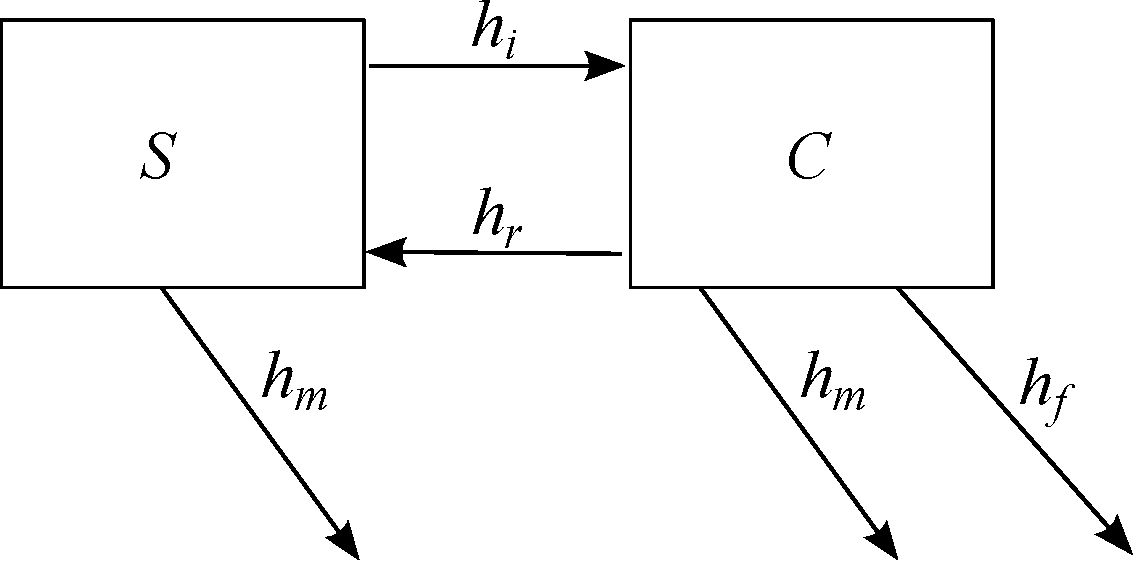
\includegraphics[width=5in]{SC.pdf}
            \caption{The two-compartment model of process for disease in a population, around which the metaregression framework is built. Compartment $S$ contains the population susceptible to the disease and compartment $C$ contains the population with the condition. Individuals move from $S$ to $C$ with incidence hazard $h_i$, and from $C$ to $S$ with remission hazard $h_r$. The susceptible population flows out of the system with without-condition mortality hazard $h_m$, and the with-condition population flows out of the system with with-condition mortality hazard $h_m+h_f$, where $h_f$ is the excess mortality hazard, representing quantitatively the increase in mortality for individuals with the condition.}
            \label{forward-sim-two-compartment}
        \end{center}
    \end{figure}

The precise mathematical representation of this model will be
elaborated on in great detail in
Chapter~\ref{forward-simulation}. Without going into details, it is
intuitive that there must be a relationship between
incidence, prevalence, remission, and with-condition mortality. The
data that has been gathered for each of these epidemiological
parameters should all be brought together in a theoretically grounded
process of data confrontation to produce a best estimate and plausible
uncertainty bounds for disease incidence and prevalence, if this is to
be used in YLD estimation. Through this grand synthesis of a
meta-analysis, I hope to produce the best possible estimates of
disease burden.

